\documentclass[a4paper,norsk]{article}
\usepackage[utf8]{inputenc}
\usepackage[T1]{fontenc,url}
\usepackage{babel,textcomp}
\usepackage{graphicx, wrapfig}
\usepackage{graphics}
\graphicspath{
	{Code/figs/}
	{Code/scorefigs/}
}
\usepackage{amsmath}
\usepackage{stackengine}
\usepackage{listings}
\usepackage{amsfonts}
\urlstyle {sf}
\title {Project 1 FYS-STK4155 Autumn 2017}
\author {Jon Audun Baar \& Mikael Ravndal}
\begin{document}
\maketitle
All of the plots of the models are done with degree equals 5.
\section*{Introduction}
In this project we were to analyse different sets of data; test-data from the Franke-function and real data, using different linear regression models. The main goal of the project was to evaulate the different models, and come to a conclusion in terms of which models would fit best with which data.
\\Most of our code is in the GitHub repository. We have chosen to not use the code in our report.
\\We have, however, made a python file, project01.py, that provides most of our code in sequence, so that it is possible to follow the code that produce our tests and plots in order.
\section*{Ordinary least square on test data}
First we have generated some test data, with the noise being very little, which we have plotted to get a more intuitive feel for how it looks. We have done this for all the models.
\\Ordinary Least square of the Frankefunction(the same as Ridge with $\lambda=0$):
\\ 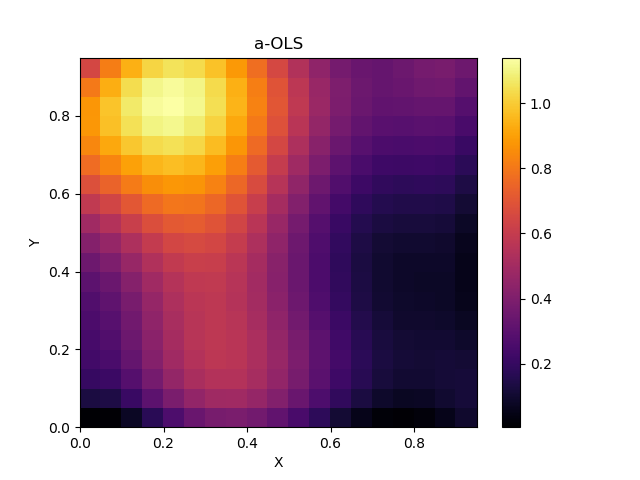
\includegraphics[scale=.7]{a-OLS}
\\As you can tell from our code, we haven't made an own function for ordinary least square, since it is the same as Ridge, just with the $\lambda$ set to 0. This will also show later that when the $\lambda$ gets low it is very similar to OLS.
\\Here is the values for calculating the five first degrees and their MSE and  R2-score:
\\OLS Test Data
\begin{table}[!h]
\begin{tabular}{lll}
k & MSE                   & R2                 \\
1 & 0.020836568820240136  & 0.7159598591230791 \\
2 & 0.015631136506458913  & 0.7869193218104034 \\
3 & 0.007175355204257789  & 0.9021869233537347 \\
4 & 0.003960217232650187  & 0.9460150723293508 \\
5 & 0.0018602479352178107 & 0.9746414541595732
\end{tabular}
\end{table}
We can tell that our model is fitting our test data better and better with a higher degree. Now we have to check with bootstrap as well to see if our model fits the data good.
\\Before the resampling we have also calculated the betas of $k=5$:
\\Var of Beta, degree 5
\begin{align*}
[9.47238055e-03\quad 8.01217226e-01 \quad4.12183842e-01\quad 9.89887798e+00\\
8.39455751e+00\quad 4.14211294e+00\quad 2.71771303e+01\quad 3.28888083e+01\\
1.78285914e+01\quad 1.31093669e+01\quad 1.91368860e+01\quad 2.67004422e+01\\
1.91391193e+01\quad 9.34737951e+00\quad 1.13215581e+01\quad 2.55450522e+00\\
4.40599813e+00\quad 3.60735967e+00\quad 1.80107762e+00\quad 1.00979408e+00\\
1.50021893e+00]
\end{align*}
Also the 95-percentage confidence interval of the betas:
95-percentage CI of betas, degree 5
\begin{align*}
[[ 7.25873511e-02\quad  4.54098870e-01]\\
[ 7.23335269e+00\quad  1.07421092e+01]\\
[ 3.44378188e+00 \quad 5.96043621e+00]\\
[-4.41211552e+01\quad -3.17880887e+01]\\
[-2.42828028e+01\quad -1.29254533e+01]\\
[-1.57022805e+01\quad -7.72437196e+00]\\
[ 4.22571363e+01\quad  6.26923830e+01]\\
[ 4.18269196e+01\quad  6.43072224e+01]\\
[ 1.67482166e+01\quad  3.32996879e+01]\\
[-1.02120404e+01\quad  3.98078784e+00]\\
[-3.30453851e+01\quad -1.58973753e+01]\\
[-7.33667324e+01\quad -5.31114961e+01]\\
[-1.94596236e+01\quad -2.31061330e+00]\\
[-3.98768180e+01\quad -2.78922323e+01]\\
[ 1.90552365e+01\quad  3.22448231e+01]\\
[-2.43921072e+00\quad  3.82593943e+00]\\
[ 1.88142647e+01\quad  2.70423776e+01]\\
[ 8.68290825e+00\quad  1.61280472e+01]\\
[-7.84195698e+00\quad -2.58124771e+00]\\
[ 1.66275865e+01\quad  2.05666637e+01]\\
[-1.80168037e+01\quad -1.32155417e+01]]\\
\end{align*}
\\ The code and commenting for the calculations is to be found in python-file project01.py
\subsection*{Resampling}
Using our bootstrapping algorithm with a resampling of 100, degree of five, we get these values:

VAR: 0.000052
\\BIAS: 0.001933
\\Bootstrap mean of MSE: 0.0020
\\Bootstrap mean of r2Score: 0.9757
\\ 
\\The bootsrap values aligns pretty well with our original ones.
\clearpage
\section*{Ridge regression}
Ridge Regression with $\lambda = 0.1$
\\Graphic plot of how it looks:
\\ 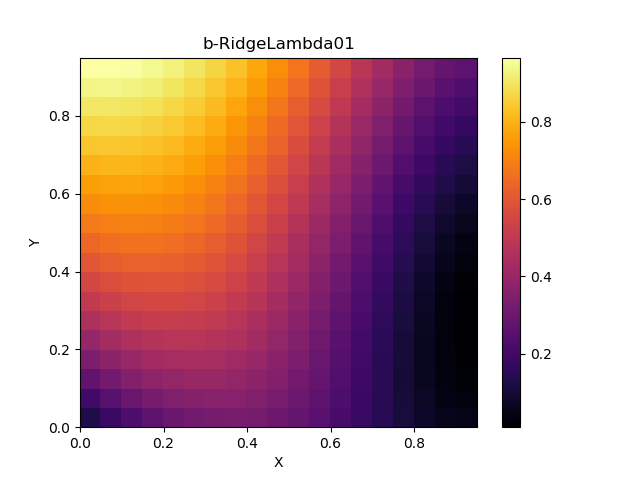
\includegraphics[scale=.7]{b-RidgeLambda01}
\\Ridge Test Data
\begin{table}[!h]
\begin{tabular}{lll}
k & MSE                   & R2                 \\
1 & 0.025965982389446095  & 0.6906471643146342 \\
2 & 0.018247163430545398  & 0.7826074259086047 \\
3 & 0.010258352759015437  & 0.8777843076427536 \\
4 & 0.009382588378732645  & 0.8882179662029949 \\
5 & 0.009143926633340667 & 0.8910613282063765
\end{tabular}
\end{table}
\\Compared to OLS, we can tell that Ridge does significantly worse then OLS.

\subsection*{Resampling}
We can take a look at how different lambdas and different degrees of the polynomial makes a change in the R2-score and the MSE.
\\Here is a plot to show how they develop as a function of lambda.
\\ 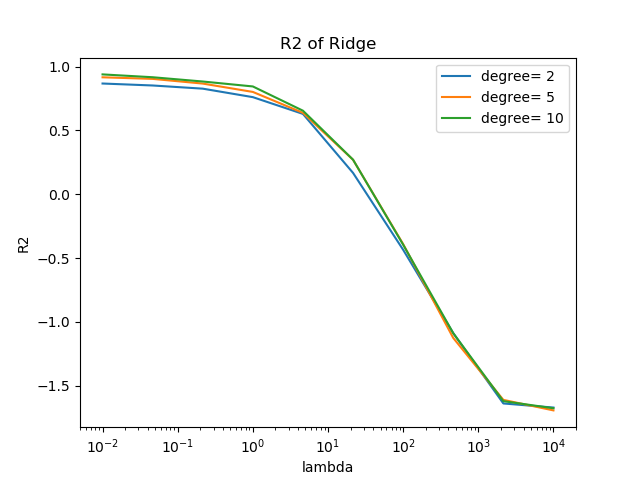
\includegraphics[scale=.7]{R2Ridge}
\\ We can tell pretty easily that the degree of the predictions doesn't matter much compared to how much the choice of lambda do. We can still tell that a lower degree function does worse then the other functions.

\clearpage

\section*{Part c)}
Lasso Regression with $\lambda = 0.01$
\\ 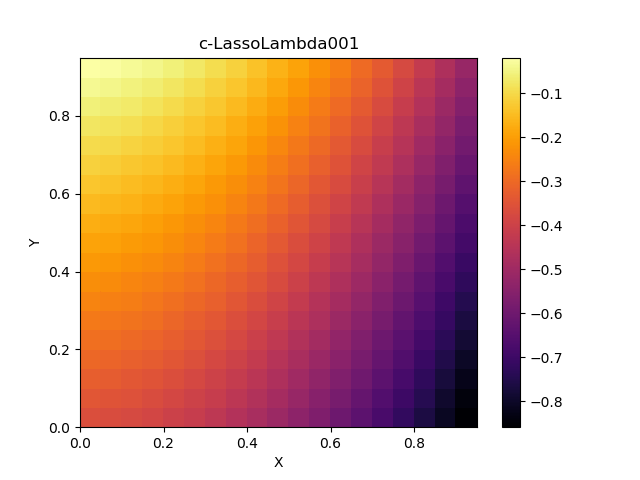
\includegraphics[scale=.7]{c-LassoLambda001}
\clearpage

\section*{Part d)}
Imports 100x100 chunk of real data from top left corner of dataset nr.1.
\\Plot of real data
\\ 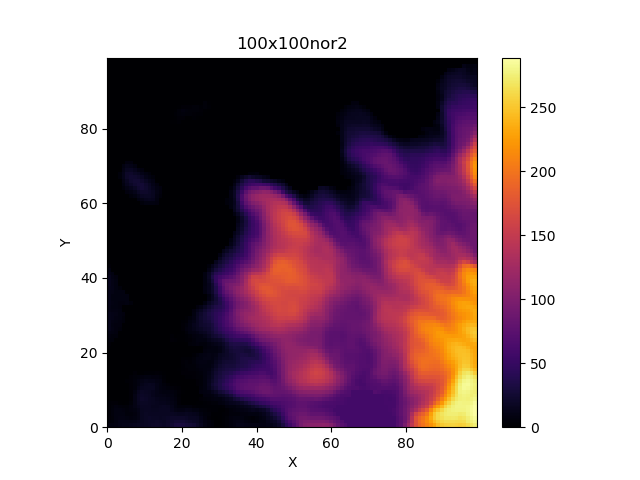
\includegraphics[scale=.7]{100x100nor2}
\clearpage
\section*{Part e)}
Repeat of a-c, but with real data from d)
\\OLS:
\\ 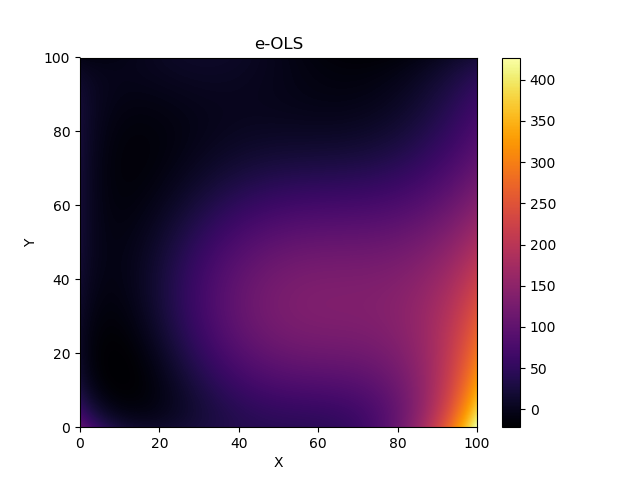
\includegraphics[scale=.7]{e-OLS}
\\Ridge:
\\ 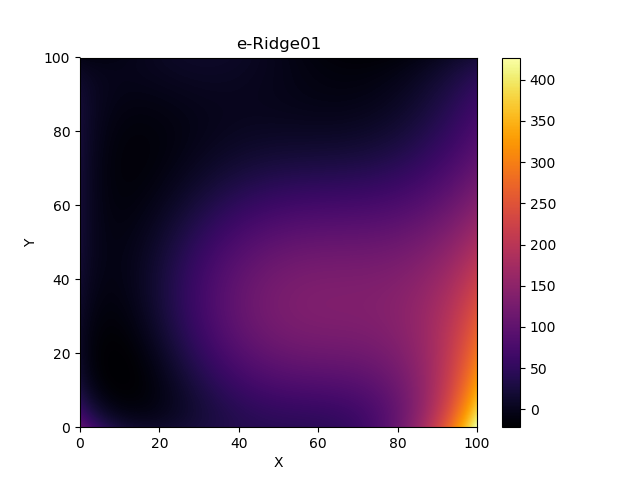
\includegraphics[scale=.7]{e-Ridge01}
\\Lasso:
\\ 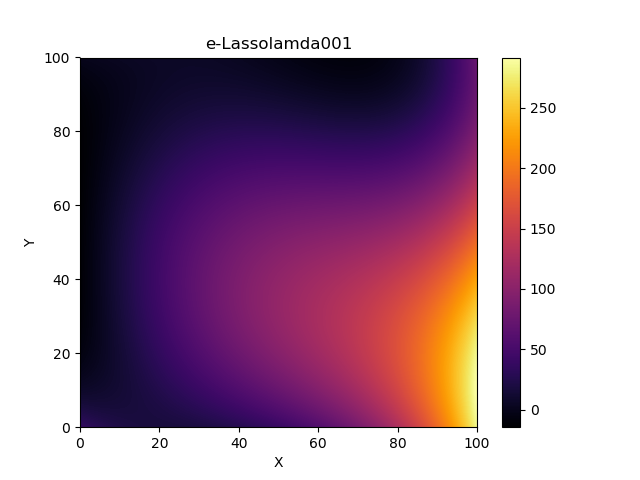
\includegraphics[scale=.7]{e-Lassolamda001}
\end{document}
